% Numerisches und Symbolisches Rechnen Zusammenfassung
% aus dem Informatikstudium an der ETH Zuerich
% basierend auf der Vorlesung von Prof. Petros Koumoutsakos 
% Copyright (C) 2003  Patrick Pletscher

\documentclass[german, 10pt, a4paper, twocolumn]{scrartcl}

\usepackage{babel}
\usepackage{amsmath}
\usepackage{amsfonts}
\usepackage{makeidx}
\usepackage[pageanchor=false,colorlinks=true,urlcolor=black,hyperindex=false]{hyperref}
\usepackage[bf]{caption2}
\usepackage[dvips]{graphicx}
\renewcommand{\captionfont}{\small\itshape}
\renewcommand{\figurename}{Abb.}

\textwidth = 19 cm
\textheight = 25 cm
\oddsidemargin = -1.5 cm
\evensidemargin = -1.5 cm
\hoffset = 0.0 cm
\marginparwidth = 0.0 cm
\topmargin = -1.0 cm
\headheight = 0.0 cm
\headsep = 0.0 cm
\parskip = 0 cm
\parindent = 0.0 cm

\makeindex
\newtheorem{theorem}{Theorem}

% Tiefe des Inhaltsverzeichnisses
\setcounter{secnumdepth}{2}
\setcounter{tocdepth}{2}

\title{Numerisches und Symbolisches Rechnen - Zusammenfassung}
\author{Patrick Pletscher}
\begin{document}

\maketitle

\section{Function Fitting}
\index{Function Fitting}

\textit{Gegeben}: N Datenpunkte $\{x_i,y_i\},\:i=1\ldots N$\\
\textit{Gesucht}: Funktion $f(x)$ welche die Punkte approximiert\\
\textit{Ansatz}:
\begin{equation}
 f(x)=\sum^M_{k=1}\alpha_k\phi_k(x)
 \label{function_fitting_ansatz}
\end{equation}

Dabei hat die approximierte Funktion M Parameter.

\subsection{Lagrange Polynome}

\index{Lagrange Polynome}

Falls $M=N$, also die Funktion gleich viele Parameter wie es Datenpunkte gibt, haben soll.

\begin{displaymath}
	\l_k(x)=\frac{(x_1-x)\ldots(x_{k-1}-x)(x_{k+1}-x)\ldots(x_N-x)}{(x_1-x_k)\ldots(x_{k-1}-x_k)(x_{k+1}-x_k)\ldots(x_N-x_k)}
\end{displaymath}

F"ur unseren Ansatz ~(\ref{function_fitting_ansatz}) setzen wir:\\
$\phi_k=l_k$\\
$\alpha_k=y_k$

\index{St"utzstelle}

Das Polynom $l_k(x)$ nimmt an jeder St"utzstelle $x_k$ genau den Wert $y_k$ an, bei den anderen St"utzstellen ist das Polynom gleich 0.\\
Diese Methode eignet sich nur bei Daten, von denen man weiss, dass sie \textit{polynomiell verteilt} sind, und \textit{kein Rauschen} enthalten.\\\\

\index{Lagrange Polynome, Fehler}

Fehler der Lagrange Polynome:
\begin{displaymath}
	|y(x)-f(x)|=|\frac{y^n(\xi)}{n!}\prod^n_{k-1}(x-x_k)|
\end{displaymath}

\subsection{Linear Least Squares}

\index{Linear Least Squares}

Falls $M<N$ verwendet man wieder den Ansatz ~(\ref{function_fitting_ansatz}).\\
\textit{Voraussetzung}: $\phi_k$ ist linear in $\alpha_k$ (also z.Bsp. nicht: $e^{\alpha_k x}$)

\begin{displaymath}
\left (
\begin{array}{cccc}
 \phi_1(x_1) &	\phi_2(x_1) &	\ldots &	\phi_M(x_1)\\
 \phi_1(x_2) &	\phi_2(x_2) &	\ldots &	\phi_M(x_2)\\
 \vdots &	\vdots &	\vdots &	\vdots\\
 \phi_1(x_N) &	\phi_2(x_N) &	\ldots &	\phi_M(x_N)
\end{array}
\right )
\left(
\begin{array}{c}
 \alpha_1\\
 \vdots\\
 \alpha_M
\end{array}
\right ) =
\left (
\begin{array}{c}
 y_1\\
 y_2\\
 \vdots\\
 y_N
\end{array}
\right )
\end{displaymath}
\begin{displaymath}
	\mathbf{A}\mathbf{x}=\mathbf{b}
\end{displaymath}

Dieses System ist "uberbestimmt und nicht exakt l"osbar.\\

\textit{L"osung}:
\begin{displaymath}
	\mathbf{A}^T\mathbf{Ax}=\mathbf{A}^T\mathbf{b}
\end{displaymath}

Falls die Kolonnen von A \textit{linear unabh"angig} sind, so ist $\mathbf{A}^T\mathbf{A}$ invertierbar und es gilt:

\begin{displaymath}
	\mathbf{x}=(\mathbf{A}^T\mathbf{A})^{-1}\mathbf{A}^T\mathbf{b}
\end{displaymath}

\textit{Beispiel}:\\
Zu approximierende Funktion: $y=ax^2+bx+c$\\
Punkte:
\begin{tabular}[ht]{l|llll}
 x & 1 & 2 & 3 & 4\\ \hline
 y & 3 & 6 & 8 & 11
\end{tabular}

\begin{displaymath}
\mathbf{A}=
\left (
\begin{array}{ccc}
 1 & 1 & 1\\
 4 & 2 & 1\\
 9 & 3 & 1\\
 16 & 4 & 1
\end{array}
\right ),\: \mathbf{b}=
\left (
\begin{array}{c}
 3 \\
 6 \\
 8 \\
 11 
\end{array}
\right )
\end{displaymath}

\subsubsection{LLS und orthonormale Matrizen}

\index{LLS und orthonormale Matrizen}

Da f"ur Matrizen mit orthonormalen Kolonnen gilt:
\begin{displaymath}\mathbf{Q}^T\mathbf{Q}=I=\mathbf{Q}\mathbf{Q}^T\end{displaymath}
\begin{displaymath}\mathbf{Q}^T=\mathbf{Q}^{-1}\end{displaymath}

Jede Matrix $\mathbf{A}$ mit linear unabh"angigen Kolonnen kann faktorisiert werden in $\mathbf{A}=\mathbf{QR}$, wobei $\mathbf{Q}$ orthonormal ist und $\mathbf{R}$ eine obere Dreiecksmatrix und invertierbar ist.\\

Somit vereinfacht sich die LLS L"osung zu folgendem Problem, falls die QR-Zerlegung der Matrix $\mathbf{A}$ bekannt ist:
\begin{displaymath}\mathbf{x}=\mathbf{R}^{-1}\mathbf{Q}^T\mathbf{b}\end{displaymath}

\subsubsection{QR-Zerlegung nach Gram-Schmidt}

\index{QR-Zerlegung}
\index{Gram-Schmidt}

Sei $\mathbf{A}=(\mathbf{a}_1 \ldots \mathbf{a}_m)$ eine Matrix mit linear unabh"angigen Kolonnen, so kann man sie wiefolgt in eine Matrix $\mathbf{QR}$ zerlegen.\\

$\mathbf{Q}$:\\
$
\begin{array}{c}\mathbf{q}_1=\frac{\mathbf{a}_1}{\|\mathbf{a}_1\|}\end{array}\\
\left.\begin{array}{l}
 \widetilde{\mathbf{q}_k}=\mathbf{a}_k-\sum^{k-1}_{j=1}\mathbf{q}_j\langle \mathbf{q}_j, \mathbf{a}_k\rangle\\
 \mathbf{q}_k=\frac{\widetilde{\mathbf{q}_k}}{\|\widetilde{\mathbf{q}_k}\|}
\end{array}
\right \} k=2,\ldots,n
$\\

$\mathbf{R}$:\\
$
\begin{array}{l}r_{11}=\|\mathbf{a}_1\|\end{array}\\
\left.\begin{array}{l}
r_{jk}=\langle \mathbf{q_j},\mathbf{a_k}\rangle ,\quad j=1,\ldots,k-1\\
r_{jk}=0,\quad j=k+1,\ldots,n\\
r_{kk}=\|\widetilde{\mathbf{q}_k}\|
\end{array} \right \} k=2,\ldots,n
$

\subsection{Pseudoinverse und Singul"arwertzerlegung (SVD)}

\index{Pseudoinverse}

\subsubsection{Pseudoinverse}

\textit{Gegeben}: $\mathbf{Ax}=\mathbf{b}$\\

Falls die Kolonnen von $\mathbf{A}$ linear abh"angig sind, so kann man das LLS Verfahren nicht anwenden, da somit $(\mathbf{A}^T\mathbf{A})^{-1}$ nicht berechnet werden kann.\\

Es gibt aber ein anderes Verfahren, das auch auf solche Matrizen anwendbar ist:\\

\textit{L"osung}: $\mathbf{x}=\mathbf{A}^{+}\mathbf{b}$, wobei $\mathbf{A}^{+}$ die Pseudoinverse von A ist\\

\textit{Bestimmung der Pseudoinversen}\\
\begin{enumerate}
 \item $\mathbf{A}$ hat nur Eintr"age in der Diagonalen\\
  \begin{displaymath}
   \mathbf{A}=\left (
   \begin{array}{cccc}
    \sigma_1 &	0 &		\hdots &	0 \\
    0 &		\ddots&		\ddots &	\vdots\\
    \vdots &	\ddots &	\ddots &	0\\
    0 &		\hdots &	0 &		\sigma_r\\
    0 &		\hdots &	\hdots &	0\\
    \vdots &	\vdots &	\vdots &	\vdots\\
    0 &		\hdots &	\hdots &	0
   \end{array}
  \right )
  \end{displaymath}
  \begin{displaymath}
  \mathbf{A}^{+}=\left (
   \begin{array}{cccccc}
    1/\sigma_1 &	\hdots &	0 &		0 &	\hdots &	0\\
    \vdots &	\ddots &	\vdots &	0 &	\ddots &		0\\
    0 &		\hdots &	1/\sigma_r &	0 &	\hdots &	0\\
   \end{array}
  \right )
  \end{displaymath}
  $\mathbf{A}^+$ wird also bestimmt in dem man die Transponierte $\mathbf{A}^T$ von $\mathbf{A}$ bestimmt und danach von allen Diagonalelementen die Inverse bestimmt, dabei wird aber $1/0=0$ gesetzt, falls $\sigma_i=0$.
 \item $\mathbf{A}$ allgemeine NxM Matrix\\
  Man zerlegt die Matrix $\mathbf{A}$ mit der Singul"arwertzerlegung in eine Matrix der Form $\mathbf{A}=\mathbf{U}\mathbf{\Sigma}\mathbf{V}^T$, wobei
  \begin{itemize}
  	\item $\mathbf{U}$ eine MxM orthonormale Matrix ist. 
  	\item $\mathbf{V}$ eine NxN orthonormale Matrix ist. 
  	\item $\mathbf{\Sigma}$ eine NxM Matrix mit spezieller Diagonalform ist. 
  \end{itemize}
  Danach ist die Pseudoinverse wie folgt zu bestimmen:\\
  \begin{displaymath}
  	\mathbf{A}^+ = \mathbf{V}\mathbf{\Sigma}^+\mathbf{U}^T
  \end{displaymath}
  Wobei $\mathbf{\Sigma}$ die Form von Fall 1 hat und sich demnach davon leicht die Pseudoinverse bestimmen l"asst.
\end{enumerate}

\subsubsection{Singul"arwertzerlegung}

\index{Singul"arwertzerlegung (SVD)}

$\mathbf{\Sigma}$:\\
\begin{displaymath}
	\Sigma = \left (
		\begin{array}{cc}
			\Sigma_r &	0\\
			0 &		0\\
		\end{array}
	\right )
\end{displaymath}

wobei $\mathbf{\Sigma_r}=diag\{\sigma_1,\ldots,\sigma_r\}$, dessen Diagonalelemente positiv und alle gr"osser gleich geordnet sind und $\sigma_i=\sqrt{\lambda_i(\mathbf{A}^T\mathbf{A})}$, wobei $\lambda_i(\mathbf{A}^T\mathbf{A})$ die Eigenwerte von $\mathbf{A}^T\mathbf{A}$ bezeichnet.\\

$\mathbf{V}$:\\
\begin{displaymath}
	\mathbf{V}=\left (
		\mathbf{v_1},\ldots,\mathbf{v_N}
	\right )
\end{displaymath}

wobei $\mathbf{v_i}$ die normierten Eigenvektoren von $\mathbf{A}^T\mathbf{A}$ sind.\\

$\mathbf{U}$:\\
\begin{displaymath}
	\mathbf{U}=\left (
		\mathbf{u_1},\ldots,\mathbf{u_M}
	\right )
\end{displaymath}

wobei $\mathbf{u_i}$ die normierten Eigenvektoren von $\mathbf{A}\mathbf{A}^T$ sind.

\subsection{Newton Iteration}

\subsubsection{Newton Iteration in 1D}

\index{Newton Iteration in 1D}

\textit{Gesucht}: Nullstellen von $f(x)$, also $f(x)=0$ l"osen.\\

\textit{Ben"otigt}: $f(x)$, $f'(x)$ und Startwert $x_0$.\\

\textit{Iteratives Verfahren}:

\begin{displaymath}
	x_{k+1} = x_k - \frac{f(x_k)}{f'(x_k)}
\end{displaymath}

\subsubsection{Newton f"ur Systeme von nicht linearen Gleichungen}

\index{Newton f"ur Systeme von nicht linearen Gleichungen}

\textit{Gegeben}: $\mathbf{f}(\mathbf{x}):\qquad \mathbb{R}^n \to \mathbb{R}^n$

\textit{Gesucht}: Schnittpunkte von Funktionen\\

\textit{Ben"otigt}:
\begin{displaymath}
	\mathbf{f}(\mathbf{x})=\left (
		\begin{array}{c}
			f_1(\mathbf{x})\\
			\vdots\\
			f_n(\mathbf{x})
		\end{array}
	\right ),\qquad
	\mathbf{J}= \left (
		\begin{array}{ccc}
			\frac{\partial f_1}{\partial x_1} & 	\ldots &		\frac{\partial f_1}{\partial x_n} \\
			\vdots &				\vdots &		\vdots \\
			\frac{\partial f_n}{\partial x_1} &	\ldots &		\frac{\partial f_n}{\partial x_n}
		\end{array}
	\right )
\end{displaymath}
\index{Jaccobi-Matrix}

Dabei bezeichnet $\mathbf{J}$ die Jaccobi-Matrix.\\

\textit{Iteratives Verfahren}:\\
\begin{displaymath}
	\mathbf{x}_{k+1} = \mathbf{x}_k - \mathbf{J}^{-1}\mathbf{f}(\mathbf{x}_k)
\end{displaymath}

\textit{Beispiel}:

\begin{eqnarray}
	f_1(x_1,x_2) &		= &	x_1^2+x_2^2 -4 \nonumber \\
	f_2(x_1,x_2) &		= &	x_1^2-x_2^2-1
\end{eqnarray}

\begin{displaymath}
	\mathbf{J}(\mathbf{x})=\left (
		\begin{array}{cc}
			\frac{\partial f_1}{\partial x_1} &	\frac{\partial f_1}{\partial x_2} \\
			\frac{\partial f_2}{\partial x_1} &	\frac{\partial f_2}{\partial x_2}
		\end{array}
		\right ) =
		\left (
		\begin{array}{cc}
			2x_1 &	2x_2 \\
			2x_1 &	-2x_2
		\end{array}
		\right )
\end{displaymath}

\begin{displaymath}
	\mathbf{x}_0 = \left (
		\begin{array}{c}
			1.5\\
			1.5
		\end{array}
		\right )
\end{displaymath}

\begin{eqnarray}
	\mathbf{J}(\mathbf{x}_k) \mathbf{h} &	= &	-\mathbf{f}(\mathbf{x}_k) \nonumber \\
	\left (
	\begin{array}{cc}
		3 &	3 \\
		3 &	-3
	\end{array}
	\right )
	\left (
	\begin{array}{c}
		h_1\\
		h_2
	\end{array}
	\right ) &
	= &
	-\left (
	\begin{array}{c}
		2.25 + 2.25 -4\\
		2.25 - 2.25 -1
	\end{array}
	\right )\nonumber \\
	\mathbf{h} &	= & \left (
	\begin{array}{c}
		0.0833\\
		-0.25
	\end{array}
	\right )\nonumber
\end{eqnarray}

und somit gilt:

\begin{displaymath}
	\mathbf{x}_{k+1} = \left (
	\begin{array}{c}
		1.5 \\
		1.5
	\end{array}
	\right )
	+
	\left (
	\begin{array}{c}
		0.083\\
		-0.25
	\end{array}
	\right )
\end{displaymath}

\subsubsection{Newton Iteration in 1D f"ur Extremalwerte}

\index{Newton Iteration in 1D f"ur Extremalwerte}

\textit{Gesucht}: $f'(x)=0$\\

\textit{Ben"otigt}: $f'(x)$, $f''(x)$ und Startwert $x_0$.\\

\textit{Iteratives Verfahren}:

\begin{displaymath}
	x_{k+1} = x_k - \frac{f'(x_k)}{f''(x_k)}
\end{displaymath}

\subsubsection{Newton Iteration f"ur Extremalwerte einer Funktion mehrerer Variablen}

\index{Newton Iteration f"ur Extremalwerte einer Funktionen mehrerer Variablen}

$Q(\mathbf{x}):\qquad \mathbb{R}^n\to\mathbb{R}$\\

\textit{Gesucht}: $\mathbf{grad}\:Q(\mathbf{x})=\mathbf{0}$\\

\index{Hessische Matrix}

\textit{Ben"otigt}: Wir ben"otigen die Jaccobi-Matrix von $\mathbf{grad}\:Q(\mathbf{x})$, welche der Hessischen-Matrix von Q entspricht.

\begin{displaymath}
	\mathbf{hess}\: Q(\mathbf{x})=
	\left (
		\begin{array}{cccc}
			\frac{\partial^2 Q}{\partial^2 x_1} &	\frac{\partial^2 Q}{\partial x_1 \partial x_2} &	\hdots &	\frac{\partial^2 Q}{\partial x_1 \partial x_n} \\
			\frac{\partial^2 Q}{\partial x_2 \partial x_1} &	\frac{\partial^2 Q}{\partial ^2 x_2} &	&	\vdots\\
			\vdots &	&	\ddots \\
			\frac{\partial^2 Q}{\partial x_n \partial x_1} &	\frac{\partial^2 Q}{\partial x_n \partial x_2} &	&	\frac{\partial^2 Q}{\partial^2 x_n}
		\end{array}
	\right )
\end{displaymath}

\textit{Iteratives Verfahren}:

\begin{displaymath}
	x_{k+1} = x_k - (\mathbf{hess}\: Q(\mathbf{x}_k))^{T}\mathbf{grad}\: Q(\mathbf{x}_k)
\end{displaymath}

\textit{Bemerkung}: Da $\mathbf{hess}\: Q(\mathbf{x})$ symmetrisch ist (nach dem Theorem von Schwarz), muss man $\mathbf{hess}\: Q(\mathbf{x})$ nur transponieren und nicht invertieren.

\subsubsection{Non-Linear Least Squares}

\index{Non-Linear Least Squares}

\textit{Gegeben}: "Uberbestimmtes nicht lineares System $\mathbf{f}(\mathbf{x}):\: \mathbb{R}^n\to\mathbb{R}^m, \: m > n$ das man nach der Methode der kleinsten Quadrate l"osen soll.

\textit{Beispiel}:

\begin{displaymath}
	\left (
	\begin{array}{c}
		x_1^2 + x_2^2 - 4 \\
		x_1^2 - x_2^2 - 1 \\
		x_1 + x_2 -3
	\end{array}
	\right ) \approx \left (
	\begin{array}{c}
		0\\
		0 \\
		0
	\end{array}
	\right )
\end{displaymath}

Das Gauss Prinzip sagt: Finde $\mathbf{x}$ so, dass

\begin{displaymath}
	\mathbf{Q}(\mathbf{x}) = \frac{1}{2} \| \mathbf{f}(\mathbf{x}) \| _2^2 = min
\end{displaymath}

Was gleichbedeutend ist mit:

\begin{displaymath}
	\mathbf{grad} \: \mathbf{Q}(\mathbf{x}) = \mathbf{0}
\end{displaymath}

Diese Gleichung ausgedr"uckt in der Funktion $\mathbf{f}(\mathbf{x})$

\begin{displaymath}
	\mathbf{Q}(\mathbf{x})=\frac{1}{2}\sum^m_{i=1} f_i(\mathbf{x})^2
\end{displaymath}

Das kann kompakt wie folgt geschrieben werden:

\begin{displaymath}
	\mathbf{grad} \: \mathbf{Q}(\mathbf{x})=\mathbf{J}_f(\mathbf{x})^T \mathbf{f}(\mathbf{x})=\mathbf{0}
\end{displaymath}

F"ur das \textit{Beispiel} sieht die Gleichung dann wie folgt aus:

\begin{displaymath}
	\left (
	\begin{array}{ccc}
		2x_1 &		2x_2 &		1\\
		2x_1 &		-2x_2 &		1
	\end{array}
	\right )
	\left (
	\begin{array}{c}
		x_1^2 + x_2^2 -4\\
		x_1^2 -x_2^2 -1\\
		x_1 + x_2 -3
	\end{array}
	\right )
	\stackrel{!}{=} 
	\left (
	\begin{array}{c}
		0\\
		0
	\end{array}
	\right )
\end{displaymath}

Um dieses System zu l"osen gibt es nun mehrere Wege:

\begin{itemize}
	\item \textbf{Gauss-Newton Algorithmus}\\
	\index{Gauss-Newton Algorithmus}
		\begin{displaymath}
			\mathbf{x}_{k+1} = \mathbf{x}_k - (\mathbf{J}_f(\mathbf{x}_k)^T\mathbf{J}_f(\mathbf{x}_k))^{-1}\mathbf{J}_f(\mathbf{x}_k)^T\mathbf{f}(\mathbf{x}_k)
		\end{displaymath}
		Der Term $(\mathbf{J}_f(\mathbf{x}_k)^T\mathbf{J}_f(\mathbf{x}_k))^{-1}\mathbf{J}_f(\mathbf{x}_k)^T$ kommt davon, dass $\mathbf{J}_f$ nicht quadratisch ist und wir davon nicht die Inverse bestimmen k"onnen sondern nur mit LLS eine Ann"aherung an $\mathbf{J}_f^{-1}$. F"ur die Iteration k"onnen wir aber in \textsc{Matlab} den Backslash-Operator benutzen:
		\begin{enumerate}
			\item L"ose
				\begin{displaymath}
					\mathbf{J}_f(\mathbf{x}_k)\mathbf{h} = - \mathbf{f}(\mathbf{x}_k)
				\end{displaymath}
				durch
				\begin{displaymath}
					\mathbf{h} = \mathbf{J}_f(\mathbf{x}_k) \backslash -\mathbf{f}(\mathbf{x}_k)
				\end{displaymath}
			\item Iteriere
				\begin{displaymath}
					\mathbf{x}_{k+1} = \mathbf{x}_k + \mathbf{h}
				\end{displaymath}
		\end{enumerate}
		Dieses Verfahren hat eine lineare Konvergenz.
	
	\item \textbf{Newton Methode f"ur non-linear least squares}
	\index{Newton Methode f"ur NLLS}
		\begin{enumerate}
			\item L"ose
				\begin{displaymath}
					\mathbf{B} := \mathbf{J}_f^T(\mathbf{x}_k)\:\mathbf{J}_f(\mathbf{x}_k)+\sum^m_{l=1} f_l(\mathbf{x}_k)\mathbf{hess}\:f_l(\mathbf{x}_k)
				\end{displaymath}
				\begin{displaymath}
					\mathbf{B}\:\mathbf{h} = -\mathbf{J}_f(\mathbf{x}_k)^T\mathbf{f}(\mathbf{x}_k)
				\end{displaymath}
				\begin{displaymath}
					\mathbf{h} = -\mathbf{B}^{-1}\:\mathbf{J}_f(\mathbf{x}_k)^T\mathbf{f}(\mathbf{x}_k)
				\end{displaymath}
			\item Iteriere
				\begin{displaymath}
					\mathbf{x}_{k+1}=\mathbf{x}_k+\mathbf{h}
				\end{displaymath}
		\end{enumerate}
		Dieses Verfahren konvergiert quadratisch.

	\item \textbf{Steepest descent}\\
	\index{Steepest descent}
		Die Ausdr"ucke $\mathbf{B}$ in Newton und $\mathbf{J}_f(\mathbf{x}_k)^T\mathbf{J}_f(\mathbf{x}_k)$ in Gauss-Newton sind ziemlich kompliziert bzw. k"onnen teilweise nicht invertiert werden, so dass man stattdessen oft Steepest descent $\lambda \mathbf{I}$ benutzt. Dabei muss $\lambda$ aber so gew"ahlt sein, dass das Ganze konvergiert. Die Iteration sieht dann wie folgt aus:
		\begin{displaymath}
			\mathbf{x}_{k+1} = \mathbf{x}_k - \lambda \mathbf{J}_f(\mathbf{x}_k)^T \mathbf{f}(\mathbf{x}_k)
		\end{displaymath}
	
	\item \textbf{Levenberg-Marquart}
	\index{Levenberg-Marquart}
		\begin{displaymath}
			\mathbf{x}_{k+1} = \mathbf{x}_k - (\mathbf{J}_f^T\mathbf{J}_f+\lambda \mathbf{D})^{-1} \mathbf{J}_f^T\mathbf{f}(\mathbf{x}_k) 
		\end{displaymath}
		wobei $\mathbf{D}$ diagonal ist, oftmals ist $\mathbf{D}=\mathbf{I}$\\
		Praktisch wird $\mathbf{h}$ wie folgt berechnet:
		\begin{displaymath}
			\left (
				\begin{array}{c}
					\mathbf{J}_f \\
					\sqrt{\lambda} \sqrt{\mathbf{D}}
				\end{array}
			\right )
			\mathbf{h} \approx \left (
				\begin{array}{c}
					-\mathbf{f}(\mathbf{x}_k) \\
					\mathbf{0}
				\end{array}
			\right )
		\end{displaymath}
\end{itemize}

\section{Direkte Suchmethoden}
\index{Direkte Suchmethoden}

W"ahrend es bei den analytischen Methoden darum geht, das \textit{Optimum in einem Schritt} zu erreichen, ohne Test, geht es bei den Direkten Methoden darum, dass die L"osung \textit{Schritt um Schritt (iterativ)} angen"ahert wird, und bei jedem Schritt der Wert der betrachteten Funktion verbessert wird, wenn das nicht der Fall ist, so wird mit trial and error vorgegangen.

\subsection{Analytische Methoden}
\index{Analytische Methoden}

\textit{Notwenige Bedingung}: Minimiere den Gradienten - System von Gleichungen.

\index{Sattelpunkt}
\textit{Hinreichende Bedingung}:
\begin{itemize}
	\item in 1D\\
		Wenn die \textit{zweite Ableitung positiv} ist, so ist es ein \textit{Minimum}, falls \textit{negativ} ein \textit{Maximum}, und falls \textit{Null} ein \textit{Sattelpunkt}.
	\item in N-Dimensionen\\
		Die Determinate der Hessischen Matrix muss positiv sein; f"ur ein Minimum muss auch die N-1 Subdeterminate positiv sein, sonst ist es ein Maximum.\\
		Falls die Determinate der Hessischen Matrix negativ ist, so ist es ein Sattelpunkt.
\end{itemize}

\subsubsection{Die analytischen Methoden k"onnen aber auch schief gehen}

\begin{itemize}
	\item \textit{Diskontinuit"at} von der betrachteten Funktion und ihrer Ableitungen.
	\item \textit{Differentiation kann unm"oglich sein} (z.Bsp. bei Experimenten oder Black-Box Code) oder ungenau (z.Bsp. Daten mit Rauschen).
	\item Optimum kann ein \textit{Extremwert oder ein Sattelpunkt} sein.
	\item System von Gleichungen (v.a. nicht linear) kann m"oglicherweise nicht l"osbar sein oder \textit{sehr teuer} zu l"osen.
\end{itemize}

\subsection{Nicht-Gradienten basierende Methoden}

\index{Nicht-Gradienten basierende Methoden}

\subsubsection{Direkte Suchmethoden}
\index{Direkte Suchmethoden}

Wir benutzen den Ausdruck "'Direkte Suche"' um die \textit{sequenzielle Untersuchung} von Versuchen zu beschreiben. Wobei jeder Versuch mit der ''besten'' bisherigen L"osung \textit{verglichen} wird, zusammen mit einer \textit{Strategie} (als einer Funktion der bisherigen Resultate), welches der n"achste Versuch sein wird.\\
Dabei werden im Normallfall keine analytischen Betrachtungen gemacht, ausser es gibt einen grossen Vorteil.

\subsubsection{Evolutionary Operation Method (EVOP)}
\index{Evolutionary Operation Method}
\index{EVOP}

Die Schl"usselfunktion davon ist, dass sie nicht numerische Funktionswerte besitzen muss: die \textit{relative Rangierung} von Objekten ist hinreichend.\\

\textit{EVOP Algorithmus}
	\begin{enumerate}
		\item Funktion an Stellen $+d$ und $-d$ in jeder Dimension auswerten. (Am Anfang ist z.Bsp. $d = 1$)
		\item Neuer Punkt = Punkt mit minimalem Funktionswert
		\item Falls der gleiche Punkt selektiert wird, so wird $d$ skaliert (z.Bsp. verkleinert) 
		\item Iteriere bis ein $\varepsilon$ erreicht ist, oder bis zu einer maximalen Anzahl Iterationen
	\end{enumerate}

\subsubsection{Parallele Methoden}
\index{Parallele Methoden}

\begin{enumerate}
	\item Untersuche die Funktionswerte an verschiedenen Punkten
	\item Deklariere den Punkt mit dem kleinsten Funktionenwert zum Minimum
\end{enumerate}

\begin{itemize}
	\item Diese Methoden werden auch als \textit{Gitter Methoden} oder \textit{tabellarische Methoden} bezeichnet.
	\item \textit{Unglaublich langsam} - Anzahl der Versuche ist umgekehrt proportional zur Genauigkeit, aber sie sind \textit{parallel ausf"uhrbar}.
\end{itemize}

\subsubsection{Sequenzielle Methoden}
\index{Sequenzielle Methoden}

In sequenziellen Methoden:

\begin{itemize}
	\item Versuche werden \textit{sequenziell} gemacht.
	\item Zwischenresultate werden benutzt um den n"achsten Punkt zu lokalisieren.
\end{itemize}

Sie k"onnen klassifiziert werden in:

\begin{itemize}
	\item Suchmustermethoden
	\item Simplexmethoden
	\item Methoden mit lernf"ahigen Mengen von Suchrichtungen
\end{itemize}

Sind langsam, proportional zum Logarithmus der Genauigkeit

\subsubsection{Hooke und Jeeves: Exploratory Method}
\index{Hooke und Jeeves}
\index{Exploratory Method}

Eine Extrapolation entlang einer Linie von der ersten und letzten Bewegung, bevor die Variablen wieder individuell ver"andert werden.

\begin{figure}[hbt]
 \begin{center}
 	\includegraphics[width=0.4\textwidth]{hook_jeeve.eps}
 \end{center}
 \label{hook_jeeves}
 \caption{Exploratory Method nach Hooke und Jeeves}
\end{figure}

\tiny
\begin{tabular}{p{0.8cm}|p{0.6cm}|p{1cm}|p{1cm}|p{0.5cm}|p{1cm}|c}
	Nummer &	Iterat. index k &	Richtungs- index i &	Variablen- wert x1/x2 &		Vergl. punkt &		Schritt- l"ange s1/s2 &		Bemerkungen  \\ \hline
	(0) &		0 &			0 &			0 / 9 &				- &			2 / 2 &				Startpunkt \\
	(1) &		0 &			1 &			2 / 9 &				(0) &			&				success \\
	(2) &		0 &			2 &			2 / 11 &			(1) &			&				failure \\
	(3) &		0 &			2 &			2 / 7 &				(1) &			&				success \\
	(4) &		1 &			0 &			4 / 5 &				- &			2 / -2 &			extrapolation\\
	(5) &		1 &			1 &			6 / 5 &				(4),(3) &		&				success, success\\
	(6) &		1 &			2 &			6 / 3 &				(5) &			&				failure\\
	(7) &		1 &			2 &			6 / 7 &				(5) &			&				failure\\
	(8) &		2 &			0 &			10 / 3 &			-,(5) &			2 / -2 &			extrapolation
\end{tabular}
\normalsize

\subsubsection{Pattern Search Methods}

\index{Pattern Search Methods}

Ver"andere theoretische Parameter zu einer Zeit bei Schritten der \textit{gleichen Gr"osse} und wenn kein vergr"ossern oder verkleinern eines Parameters das Resultat verbessert, so \textit{halbiert man die Schrittgr"osse}.\\

Pattern search methods sind durch eine Serie von untersuchenden Bewegungen charakterisiert, welche das Verhalten der betrachteten Funktion \textit{in einem Muster von Punkten}, welche alle auf einem \textit{rationalen} Gitter liegen.\\

Die Schl"usselfunktion ist, dass die Punkte auf einem Gitter bleiben.\\

\textit{Konvergenz}:\\

\begin{theorem}[Polak]
Wenn $\{X_k\}$ eine Sequenz ist, welche von einer pattern search Methode erstellt wurde, so befriedigt jeder Ansammlungspunkt, dass
\begin{displaymath}
	\nabla f(x^*) = 0
\end{displaymath}
Die Methode kann nur eine endliche Anzahl von Zwischenpunkten erzeugen, bevor sie die Schrittgr"osse halbiert, somit kann der Algorithmus nicht bei einem Punkt stecken bleiben.
\end{theorem}

\subsubsection{Simplexmethode}
\index{Simplex}

\textit{Ein Simplex} ist eine Menge von $n+1$ Punkten in $\mathbb{R}^n$: Im 2D ein Dreieck, in 3D ein Tetraeder usw.

\textit{Simplex Algorithmus}
	\begin{enumerate}
		\item Ein initialaler Simplex wird erstellt.
		\item Ermittle den Knoten mit dem schlechtesten Fit.
		\item Spiegle den schlechtesten Knoten an der Mitte der gegen"uberliegenden Kante.
		\item Der Punkt mit dem besten Resultat wird der Mittelpunkt des n"achsten Zyklus.
		\item Iteriere bis zur maximalen Genauigkeit oder Anzahl maximaler Iterationen.
	\end{enumerate}

\begin{figure}[hbt]
 \begin{center}
 	%\includegraphics[width=0.4\textwidth]{simplex.eps}
 	\includegraphics[width=0.45\textwidth]{simplex/simplex.eps}
 \end{center}
 \label{simplex}
 \caption{Simplex Algorithmus Flowchart}
\end{figure}

F"ur die Ersetzung aller $x_i$ benutzt man:

\begin{displaymath}
	x_i = x_i + c(x_l - x_i)
\end{displaymath}

Dabei ist:\\

\small
\begin{tabular}{lp{4cm}}
	$\mathbf{x_h}$ &							schlechtester Punkt, d.h. $f(\mathbf{x_h})$ ist gr"osser als die Funktion ausgewertet bei allen anderen $\mathbf{x_i}$\\
	$\mathbf{x_s}$ &							zweit-schlechtester Punkt\\
	$\mathbf{x_l}$ &							bester Punkt\\
	$\mathbf{\hat{x}}=\frac{1}{n-1}\sum^n_{i=1}\mathbf{x_i}\: (i\neq h)$ &	Mittelwert ohne schlechtesten Punkt	
\end{tabular}
\normalsize

\begin{figure}[hbt]
 \begin{center}
 	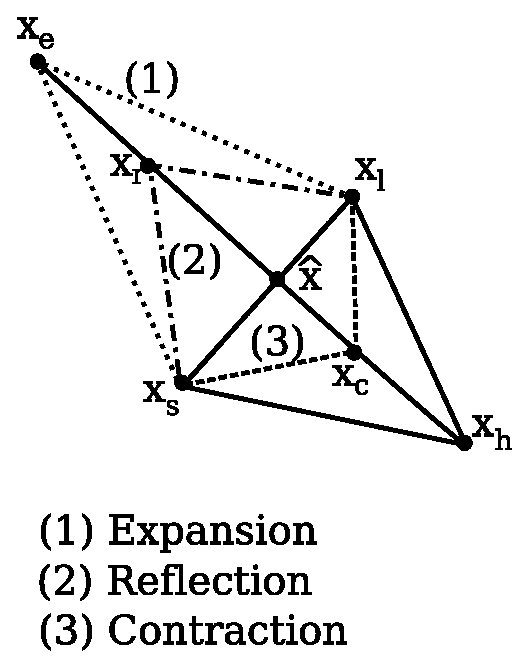
\includegraphics[width=0.25\textwidth]{simplex2.eps}
 \end{center}
 \label{simplex}
 \caption{Simplex Algorithmus grafisch}
\end{figure}

Konvergenz Kriterium:

\begin{displaymath}
	\varepsilon > \frac{\sum^n_{i=1}\sqrt{(\mathbf{x_i} - \mathbf{\hat{x}})^T (\mathbf{x_i} - \mathbf{\hat{x})}}}{n}
\end{displaymath}

\section{Fouriertransformation}
\index{Fouriertransformation}

\subsection{Fourierreihe}
\index{Fourierreihe}

Funktion f soll approximiert werden durch eine Summe von $N$ periodischen Funktionen mit je zwei Parametern:

\begin{displaymath}
	f(x) \approx \sum^N_{k=0} a_k \cos(kx) + b_k \sin(kx)
\end{displaymath}

wobei die Koeffizienten folgendermassen berechnet werden:

\begin{eqnarray}
		a_k &	 = &	\frac{1}{\pi}\int^\pi_{-\pi} f(x)\cos(kx)dx \qquad k\neq 0 \nonumber \\
		b_k &	 = &	\frac{1}{\pi}\int^\pi_{-\pi} f(x)\sin(kx)dx \nonumber \\
		a_0 &	 = &	\frac{1}{2\pi}\int^\pi_{-\pi} f(x)dx \nonumber
\end{eqnarray}

$b_0$ braucht man nicht zu betrachten, da immer gilt $b_0\sin(0)=0$.

\subsubsection{Eigenschaften der Fourierreihen}

Fehler:
\begin{displaymath}
	E = \int^\pi_{-\pi} \left [ f(x) - \sum^N_{k=0} A_k \cos(kx)+ B_k\sin(kx) \right ] ^2 dx
\end{displaymath}

Dieser Fehler wird minimiert, wenn $A_k = a_k, B_k = b_k$

\subsubsection{im Komplexen}

\begin{displaymath}
	e^{ikx} = \cos (kx) + i\sin(kx)
\end{displaymath}
\begin{displaymath}
	i^{2} = -1
\end{displaymath}

Somit ergibt sich f"ur die Fourierreihe:
\begin{displaymath}
	f(x) = \sum^\infty_{k=-\infty} c_k e^{ikx} \qquad \mbox{\&} \qquad c_k = \frac{1}{2\pi}\int_{-\pi}^\pi f(x) e^{-ikx} dx
\end{displaymath}

Wobei gilt:
\begin{eqnarray}
	c_k &	 	= & 	\frac{1}{2}a_k - \frac{1}{2}ib_k \qquad k\geq 0 \nonumber\\
	c_{-k} &	= &	\bar{c_k} = \frac{1}{2}a_k + \frac{1}{2}ib_k \nonumber \\
	a_k &		= &	c_k + c_{-k} \nonumber \\
	b_k &		= &	-\frac{1}{i}(c_k - c_{-k}) \nonumber
\end{eqnarray}

\textit{Weitere Eigenschaften}:

\begin{eqnarray*}
	\frac{d f}{d x} &	= &		ik\sum^\infty_{-\infty}c_k e^{ikx}= ikf \\
	\frac{d^2 f}{d x^2} &	= &		-k^2f  \\
	\left( \frac{d^2 }{d x^2}+\frac{d^2 }{d y^2}\right ) e^{i(k_1x +k_2y)} &	= &	-(k_1^2+k_2^2)e^{i(k_1x+k_2y)}
\end{eqnarray*}

\subsubsection{Analytische Fouriertransformation}

Die Fouriertransformierte $\hat{f}$ einer Funktion $f(x)$ ist nun wie folgt definiert:

\begin{displaymath}
	\hat{f}(k) = \int^\infty_{-\infty} f(x)e^{-ikx}dx
\end{displaymath}

Die Fouriertransformierte einer Funktion $f(x)$ wird im Nachfolgenden mit $\mathcal{F}(f)$ oder $\hat{f}(x)$

\subsection{Diskrete Fouriertransformation (DFT)}
\index{Diskrete Fouriertransformation}

Gegeben ein Datenvektor $\mathbf{x}=(x_0,x_1,\ldots,x_{N-1})$ der L"ange $n$, die DFT ist definiert als:\\

\textit{Fourier Transformation in Matrixschreibweise}:
\small
\begin{displaymath}
	\left (
		\begin{array}{ccccc}
			1 &		1 &		1 &		\ldots &		1 \\
			1 &		w &		w^2 &		\ldots &		w^{n-1}\\
			1 &		w^2 &		w^4 &		\ldots &		w^{2(n-1)}\\
			1 &		w^3 &		w^6 &		\ldots &		w^{3(n-1)}\\
			\vdots &	\vdots &	\vdots &	\vdots &		\vdots \\
			1 &		w^{n-1} &	w^{2(n-1)} &	\ldots &		w^{(n-1)^2}\\
		\end{array}
	\right )
	\left (
		\begin{array}{c}
			y_0\\
			y_1\\
			y_2\\
			y_3\\
			\vdots\\
			y_{n-1}
		\end{array}
	\right )
	=
	\left (
		\begin{array}{c}
			x_0\\
			x_1\\
			x_2\\
			x_3\\
			\vdots\\
			x_{n-1}
		\end{array}
	\right )
\end{displaymath}
\normalsize
\begin{displaymath}
	\mathbf{F} \mathbf{y} = \mathbf{x}
\end{displaymath}

Wobei das (i,j)-Element von $\mathbf{F}$ wie folgt aussieht:
\begin{displaymath}
	f_{ij} = w^{(i-1)(j-1)}
\end{displaymath}

Wobei $w$ f"ur jedes $n$ definiert ist als:
\begin{displaymath}
	w=e^{i\frac{2\pi}{n}}=e^{\frac{2\pi i}{n}} \qquad \& \qquad \bar{w} = e^{-\frac{2\pi i}{n}}
\end{displaymath}
\begin{displaymath}
	w^n=e^{2\pi i}=1
\end{displaymath}

Die DFT eines Datenvektors $\mathbf{x}$ ist nun:
\begin{displaymath}
	\mathcal{F}(\mathbf{x}) = \mathbf{y} = \frac{1}{\sqrt{n}}\mathbf{\bar{F}}\mathbf{x}
\end{displaymath}

Dabei bezeichnet $\mathbf{\bar{F}}$ die Matrix $\mathbf{F}$, wobei aber "uberall $w$ durch $\bar{w}$ ersetzt wird.\\

und die R"ucktransformation:
\begin{displaymath}
	\mathcal{F}^{-1}(\mathbf{y})=\mathbf{x}= \frac{1}{\sqrt{n}}\mathbf{F}\mathbf{y}
\end{displaymath}

\subsection{Fast Fourier Transformation}
\index{Fast Fourier Transformation}

Mit diesem Algorithmus kann die DFT effizient durchgef"uhrt werden, n"amlich in $O(n\log n)$. Gegeben ist also wieder ein Datenvektor $\mathbf{x}=(x_0,\ldots,x_{n-1})$ der L"ange $n$.
Dieser Algorithmus wird rekursiv angewendet, bis der Datenvektor $\mathbf{x}$ nur noch L"ange 1 hat, von diesem ist die Fouriertransformierte $\mathbf{y}$ dann leicht zu bestimmen, da $\mathbf{x}=\mathbf{y}$ falls die L"ange von $\mathbf{x}$ gleich 1 ist.\\

\subsubsection{Fast Fourier Transformations Algorithmus}

\begin{enumerate}
	\item Vektor $\mathbf{x}$ aufteilen in 2 Vektoren $\mathbf{x}',\mathbf{x}''$ mit geraden/ungeraden Indices
		\begin{displaymath}
			\mathbf{x}' = (x_0, x_2, x_4, \ldots, x_{n-2})
		\end{displaymath}
		\begin{displaymath}
			\mathbf{x}'' = (x_1, x_3, x_5, \ldots, x_{n-1})
		\end{displaymath}
	\item Fouriertransformierte $\mathbf{y}'=\mathbf{\bar{F}}\mathbf{x}'$ und $\mathbf{y}''=\mathbf{\bar{F}}\mathbf{x}''$  bestimmen (rekursiv mit FFT).
	\item Die beiden Vektoren $\mathbf{y}'$ und $\mathbf{y}''$ wie folgt zusammensetzen:
		\begin{displaymath}
			y_j = y_j' + \overline{w}^j_n y_j'' \qquad \mbox{f"ur }j=0,\ldots,\frac{n}{2}-1
		\end{displaymath}
		\begin{displaymath}
			y_{j+\frac{n}{2}} = y_j' - \overline{w}^j_n y_j'' \qquad \mbox{f"ur }j=0,\ldots,\frac{n}{2}-1
		\end{displaymath}
\end{enumerate}

F"ur die R"ucktransformation muss $w_n$ an Stelle von $\overline{w}_n$ gew"ahlt werden und $\mathbf{F}$ statt $\mathbf{\bar{F}}$.

\section{Faltung}
\index{Faltung}

Die Faltung zweier Funktionen $f$ und $g$, ist definiert als:
\begin{displaymath}
	f \ast g = \int_{-\infty}^{\infty} f(\xi)g(x-\xi)d\xi
\end{displaymath}

Dadurch werden die Punkte von $f(x)$ nach $g(x)$ gewichtet.\\

\textit{Eigenschaften}:
\begin{eqnarray}
	\mathcal{F}(f\ast g) &		= &		\mathcal{F}(f) \cdotp \mathcal{F}(g) \nonumber \\
	f\ast (g+ h) &			= &		(f\ast g)+ (f\ast h) \nonumber \\
	\frac{d}{dx}(f\ast g) &		= &		\frac{df}{dx}\ast g = f\ast \frac{dg}{dx} \nonumber 
\end{eqnarray}

\subsection{Diskrete Faltung}
\index{Faltung, Diskrete}

Die Funktionen sind durch Punkte $\mathbf{f}=(f_0,f_1,\ldots,f_{n-1})$ und $\mathbf{g}=(g_0,g_1,\ldots,g_{n-1})$ gegeben. Die diskrete Faltung berechnet sich wie folgt:
\begin{displaymath}
	f\ast g = \left (
			\begin{array}{c}
				f_0 g_0 + f_1 g_{n-1} + f_2 g_{n-2} + \ldots + f_{n-1} g_1 \\
				f_0 g_1 + f_1 g_{0} +f_2 g_{n-1} + \ldots +f_{n-1} g_2 \\
				\vdots\\
				f_0 g_{n-1} + f_1 g_{n-2} + f_2 g_{n-3} + \ldots + f_{n-1} g_0
			\end{array}
		\right )
\end{displaymath}

\textit{Bemerkungen}:
\begin{itemize}
	\item Das Faltungsprodukt von zwei Vektoren der L"ange n hat L"ange n.
	\item Jede Komponenete hat n Terme
	\item Kosten: $O(n^2)$
	\item Erste Komponente enth"alt alle Produkte $f_j g_k$ mit $j+k=0$ oder $j+k=n$
	\item l-te Komponente enthalten alle Produkte mit $j+k=l$ oder $j+k=l+n$
\end{itemize}

\subsubsection{Faltungsregel}

Die Faltung von $f$ und $g$ ist eine gew"ohnliche Multiplikation der Fouriertransformierten Funktionen.\\

$f\ast g$ wird berechnet:
\begin{enumerate}
	\item $c = \mathcal{F}^{-1}(f)$
	\item $d = \mathcal{F}^{-1}(g)$
	\item Multipliziere $c$ und $d$ Komponente f"ur Komponente
	\item $(f\ast g) = \sqrt{n} \cdotp \mathcal{F}(cd)$		% von wo das n?
\end{enumerate}

\subsection{$\delta$ Funktion (Dirac Funktion)}
\index{Dirac Funktion}

\subsubsection{Definition}

Wir m"ochten eine Erregung $d_a(x)$, die "uber einem kleinen Intervall $a-\varepsilon < x < a+\varepsilon$ nicht-Null ist, und sonst "uberall Null ist, beschreiben. Der gesamte Impuls davon ist dann definiert als:
\begin{displaymath}
	I = \int^\infty_{-\infty} d_a(x) dx = \int^{a+\epsilon}_{a-\epsilon} d_a(x) dx\qquad (\varepsilon > 0)
\end{displaymath}

Um ein mathematisches Modell der Funktion $d_a(x)$ zu geben, ist es bequem, anzunehmen, dass sie einen konstanten Wert "uber dem geschlossenen Intervall $[a-\varepsilon, a+\varepsilon]$ annimmt, auch m"ochten wir diesen Wert so w"ahlen, dass der Gesamtimpuls gleich 1 ist. Also schreiben wir:
\begin{displaymath}
	d_a(x) = \left \{
		\begin{array}{cc}
			\frac{1}{2\varepsilon}&		a-\varepsilon \leq x \leq a + \varepsilon \\
			0 &				\mbox{sonst}
		\end{array}
		\right .
\end{displaymath}

Nun betrachten wir eine Idealisierung der Funktion $d_a(x)$, indem wir $\varepsilon$ gegen Null gehen lassen:
\begin{displaymath}
	\lim_{\varepsilon \to 0} I = \lim_{\varepsilon \to 0}\int^\infty_{-\infty}d_a(x)dx =1
\end{displaymath}

Damit k"onnen wir eine idealisierte Ein-Puls Funktion $\delta(x-a)$ definieren, welche die Eigenschaft hat, dass sie einen Impuls von 1 bei der Stelle $x=a$ hat, aber f"ur alle anderen Werte von $x$ Null ist. Die \textit{Definitionseigenschaften} sind deshalb:
\begin{eqnarray}
	\delta(x-a) & 					= &	0 \qquad x\neq a \nonumber \\
	\int^\infty_{-\infty}\delta(x-a)dx & 		= &	1 \nonumber
\end{eqnarray}

oder f"ur $a=0$:
\begin{eqnarray}
	\delta(x) & 					= &	0 \qquad x\neq 0 \nonumber \\
	\int^\infty_{-\infty}\delta(x)dx & 		= &	1 \nonumber
\end{eqnarray}

Im weiteren wird mit $a$ gerechnet, wobei man aber nat"urlich f"ur den Fall $a=0$ $a$ weglassen kann (wie in der Vorlesung).\\

\subsubsection{Weitere Eigenschaften}

\begin{eqnarray}
	\int^\infty_{-\infty} f(x) \delta(x-a) dx &	= &		f(a) \nonumber \\
	f(x)&						= &		\int^\infty_{-\infty} f(y)\delta(y-x)dy \nonumber
\end{eqnarray}

Die $\delta$ Funktion erm"oglicht es uns eine diskrete Funktion (z.B. Datenpunkte) als kontinuierliche Funktion zu schreiben.\\

\textit{Beispiel}: Datenpunkte $\{(x_1,f_1), \ldots, (x_n,f_n)\}$ k"onnen dann als Funktion so geschrieben werden:
\begin{displaymath}
	f(x)= \sum^n_{i=1} f_i \delta (x-x_i)
\end{displaymath}

\subsection{Wichtige Fouriertransformationen und Faltungen}

\begin{enumerate}
	\item 	\begin{eqnarray}
			f(x) &		= &		\delta(x) \nonumber \nonumber \\
			\hat{f}(k) &	= &		\int^{\infty}_{-\infty} e^{-ikx}\delta(x) dx = 1 \nonumber
		\end{eqnarray}
	
	\item	\begin{displaymath}
			f(x) = \mbox{ square pulse } = \left
				\{
				\begin{array}{ll}
					1 &		-L \leq x \leq L\\
					0 &		|x| > L
				\end{array}
				\right .
		\end{displaymath}
		\begin{displaymath}
			\hat{f}(k)=\int^{L}_{-L}e^{-ikx}dx = \frac{e^{-ikL}-e^{ikL}}{-ik}=\frac{2\sin(kL)}{k}
		\end{displaymath}
	
	\item	\begin{displaymath}
			f(x) = \left
				\{
				\begin{array}{ll}
					e^{-ax} &		x > 0\\
					0 &			x < 0\\
				\end{array}
				\right .
		\end{displaymath}
		\begin{displaymath}
			\hat{f}(k)=\frac{1}{a+ik} \qquad a> 0
		\end{displaymath}
	
	\item	\begin{displaymath}
			f(x) = e^{-a|x|} \qquad a > 0
		\end{displaymath}
		\begin{displaymath}
			\hat{f}(k)= \frac{2a}{a^2+k^2}
		\end{displaymath}
\end{enumerate}

\begin{displaymath}
	\begin{array}{l}
		f(x) \dotfill \hat{f}(k) \\
		\frac{d}{dx} f(x) \dotfill ik\hat{f}(k)\\
		f(x-d) \dotfill	e^{-ikd}\hat{f}(k) \\
		e^{ixd}f(x) \dotfill \hat{f}(k-d)\\
		\qquad\qquad\qquad\qquad\qquad\qquad\qquad\qquad
	\end{array}
\end{displaymath}

\begin{displaymath}
	\hat{\delta} = 1
\end{displaymath}
\begin{displaymath}
	\hat{f} = \hat{f}\cdotp 1 = \hat{f}\cdotp\hat{\delta}
\end{displaymath}
\begin{displaymath}
	f(x) = f(x)\ast\delta(x) = \int^{\infty}_{-\infty}f(y)\delta(x-y)dy
\end{displaymath}

\subsection{Faltung und Differentialrechnung}

\textit{Gegeben}: Differentialgleichung der Form
\begin{displaymath}
	L u(x) = h(x)
\end{displaymath}

Wobei L ein Differentialoperator ist, (z.Bsp. $L=-\frac{d}{dx^2}+a^2$ oder $L=\frac{d}{dx}$).\\

\begin{enumerate}
	\item Forme die ganze Gleichung in den Fourierraum um, dabei ersetzt man am besten die rechte Seite durch $h(x)$, bzw. nach dem Transformieren durch $\hat{h}(k)$ und benutzt die Regel f"ur das Transformieren einer Ableitung:
		\begin{displaymath}
			\mathcal{F}\left(\frac{df}{dx} \right) = ik\mathcal{F}(f)
		\end{displaymath}
	\item Man hat nun einen Ausdruck der Form
		\begin{displaymath}
			\hat{u}(k) = \hat{f}(k)\cdotp\hat{g}(k)
		\end{displaymath}
		Dabei ist $\hat{g}(k)$ die sogenannte "'Green's function"'.
	\item Berechne nun dieses Produkt im Fourierraum, somit erh"alt man $\hat{u}(k)$.
	\item Transformiere $\hat{u}(k)$ zur"uck in den Realspace.
\end{enumerate}

\textit{Beispiel}:
\begin{eqnarray}
	\mathcal{F}\left(-\frac{d^2 u}{dx^2}+a^2 u(x) \right ) &= &		\mathcal{F}(h(x))		\nonumber \\
	-(ik)^2\hat{u}(k) + a^2\hat{u}(k) &			= &		\hat{h}(k)	\nonumber \\
	k^2\hat{u}(k) + a^2\hat{u}(k) &				= &		\hat{h}(k)	\nonumber \\
	\hat{u}(k) &						= &		\frac{\hat{h}(k)}{a^2+k^2} = \hat{h}(k)\cdotp \hat{g}(k)	\nonumber
\end{eqnarray}

Jetzt m"usste man $\hat{u}(k)$ noch zur"ucktransformieren.

\section{Principal Component Analysis}
\index{Principal Conmponent Analysis}

\begin{figure}[hbt]
 \begin{center}
 	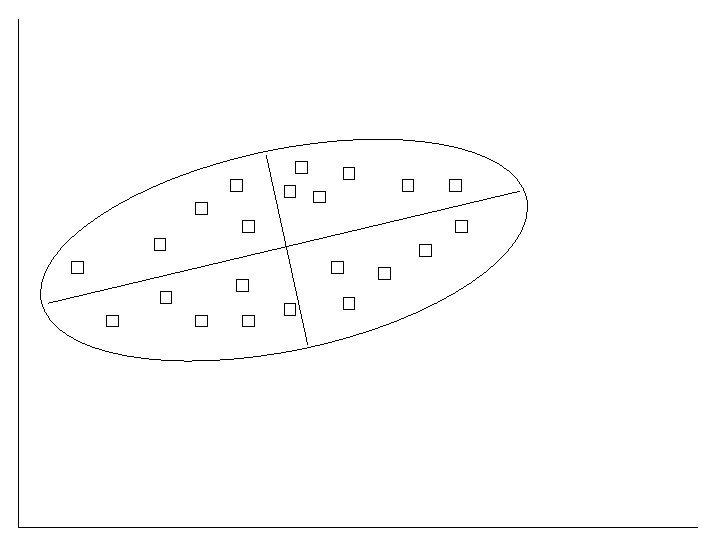
\includegraphics[width=0.25\textwidth]{principalcomp.eps}
 \end{center}
 \label{principal_components}
 \caption{Steigung der Halbachsen beschreibt die Punkte}
\end{figure}

\subsection{Statistische Ausdr"ucke}

Mittelwert:
\begin{displaymath}
	\bar{x} = \frac{1}{n}\sum^n_{i=1} x_i
\end{displaymath}

Varianz:
\begin{displaymath}
	s^2 = \frac{1}{n-1}\sum^n_{i=1}(x_i-\bar{x})^2
\end{displaymath}

Standardabweichung:
\begin{displaymath}
	s = \sqrt{s^2}
\end{displaymath}

Kovarianz:
\begin{displaymath}
	cov(X,Y) = \frac{\sum^n_{i=1}(x_i-\bar{x})(y_i-\bar{y})}{n-1}
\end{displaymath}

F"ur mehrdimensionale Daten erstellen wir die Kovarianz-Matrix:
\begin{displaymath}
	Cov(x,y,z) = 	\left (
				\begin{array}{ccc}
					cov(x,x) &	cov(x,y) &	cov(x,z)\\
					cov(y,x) &	cov(y,y) &	cov(y,z)\\
					cov(z,x) &	cov(z,y) &	cov(z,z)
				\end{array}
			\right )
\end{displaymath}

\textit{Rechenregeln}
\begin{enumerate}
 \item $var(X+Y)=var(X)+var(Y)$ wenn $X,Y$ unabh.
 \item $var(N(0,1))=1$
 \item $cov(X,Y) = 0$ wenn $X,Y$ unabh.
 \item $cov(X,X)=var(X)$
 \item $cov(X,Y)=cov(Y,X)$
 \item $cov(aX,Y)=a\cdotp cov(X,Y)$
 \item $cov(X+Y,Z)=cov(X,Z)+cov(Y,Z)$
 \item $cov(X+Y,Z+W)=cov(X,Z)+cov(X,W)+cov(Y,Z)+cov(Y,W)$
\end{enumerate}

\subsection{Principal Components Analysis}

Ziel ist es Daten (mit Verlust) zu komprimieren, ohne aber wesentliche Daten zu verlieren.\\

$\mathbf{x}$ soll eine Menge von Messvektoren sein (also eigentlich eine Matrix) und $\mathbf{y}=\mathbf{M}\mathbf{x}$ eine Transformation vom Vektor $\mathbf{x}$ zu einem neuen Vektor $\mathbf{y}$ mit gew"unschten Eigenschaften (welche definiert werden m"ussen).\\

Die Kovarianzmatrix von $\mathbf{y}$ ist definiert durch:
\begin{displaymath}
	\mathbf{C}_y = \langle (\mathbf{y}-\langle \mathbf{y} \rangle) \cdotp (\mathbf{y}-\langle \mathbf{y} \rangle)^T\rangle
\end{displaymath}

Dabei ist $\langle \rangle$ der ensemble average, also der Mittelwert der Vektoren bzw. Matrizen.\\

Durch Umformen erh"alt man:
\begin{displaymath}
	\mathbf{C}_y = \mathbf{M} \mathbf{C}_x \mathbf{M}^T
\end{displaymath}

Nun m"ochten wir die Transformation $\mathbf{M}$ so w"ahlen, dass $\mathbf{C}_y$ diagonal ist und die Elemente unkorreliert sind:\\

$\mathbf{C}_x$ ist symmetrisch und hat eine orthonormale Menge von Eigenvektoren $q_1,\ldots,q_n$. Wir setzen die Spalten von $\mathbf{M}^T$ gleich diese Eigenvektoren.

\begin{displaymath}
	\mathbf{C}_x \mathbf{M}^T = C_x \cdotp (q_1, \ldots, q_n) = (\lambda_1 q_1, \ldots, \lambda_n q_n)
\end{displaymath}
\begin{displaymath}
	\mathbf{M}\mathbf{C}_x\mathbf{M}^T = 	\left (
							\begin{array}{ccc}
								\lambda_1 &	&		0\\
								 &		\ddots &	\\
								 0 &		&		\lambda_n
							\end{array}
						\right ) = \mathbf{C}_y
\end{displaymath}

Falls es Korrelationen zwischen den Elementen von $\mathbf{x}$ gibt, so werden einige Eigenwerte verschwinden, diese Komponenten von $\mathbf{y}$ k"onnen dann f"ur weitere Betrachtungen weggelassen werden.\\

F"ur reale Daten werden die korrelierten Eigenwerte nicht genau Null sein, aber man kann durch die relative Gr"osse die wichtigen herauslesen und die unwichtigen weglassen. Solches selektieren von Variablenuntermengen ist oftmals der Schl"ussel zu erfolgreichem Modellieren.

\subsubsection{Algorithmus}

\begin{enumerate}
	\item Daten in Matrizen oder Vektoren konvertieren. Bei Matrizen ist es bequemer, wenn man sie in Vektoren umformt und am Ende wieder zur"uck. Mehrere solcher Messvektoren (hier $n$ Messungen) der Dimension $m$ werden in einer Matrix $\mathbf{D}$ (hier spaltenweise) angeordnet.
	\item Den Mittelwertvektor $\mathbf{avg}$ bilden: 
		\begin{displaymath}
			avg_i = \frac{1}{n-1}\sum^n_{j=0} d_{ij} \qquad \text{f"ur } j = 0, \ldots, m-1
		\end{displaymath}
	\item Von jedem Messvektor den normalisierten Mittelwertvektor subtrahieren. Dies ergibt uns die normalisierte Matrix $\mathbf{D}_{norm}$
	\item Kovarianzmatrix von $\mathbf{D}_{norm}$ bilden
		\begin{displaymath}
			\mathbf{C} = \frac{1}{n-1} \mathbf{D}_{norm} \cdotp \mathbf{D}_{norm}^T
		\end{displaymath}
	\item Eigenwerte $\mathbf{E}$ und -vektoren $\mathbf{V}$ von $\mathbf{C}$ bestimmen
	\item Bestimmte Eigenvektoren $\mathbf{v}$ w"ahlen, andere nicht, z.B. die Eigenvektoren wo die Eigenwerte ungleich Null sind. Durch die gew"ahlten Eigenvektoren ergibt sich eine neue Matrix $\mathbf{Q}$.
\end{enumerate}

Um nun einen Datenvektor $\mathbf{x}$  zu komprimieren benutzt man
\begin{displaymath}
	\mathbf{y} = \mathbf{Q}^T \mathbf{x}
\end{displaymath}

F"ur die R"ucktransformation gilt
\begin{displaymath}
	\mathbf{x}' = \mathbf{Q} \mathbf{y}
\end{displaymath}

\section{Nicht lineare Gleichungen}

\subsection{Bisektion}
\index{Bisektion}

\textit{Gegeben}: $f(x)$ stetig in $[a,b]$, wobei $f(a) < 0$ und $f(b) > 0$. Daraus folgt: $\exists s: f(s)=0,\: s\in[a,b]$.\\

\textit{Gesucht}: Eine Nullstelle von $f(x)$.

\subsubsection{Bisektionsalgorithmus}

\begin{enumerate}
	\item $x := (a+b)/2$ /* x = Mitte von Intervall*/
	\item Wenn $f(x)>0, b\ := x;$ sonst $a:=x;$ /* Intervall neu */
	\item Wiederhole Algorithmus, falls $b-a > \varepsilon$, also die gew"unschte Genauigkeit noch nicht erreicht wurde
\end{enumerate}

\subsubsection{Konvergenz}

Der Bisketionsalgorithmus konvergiert linear, da der Fehler in jedem Schritt maximal $\varepsilon < (b-a)\frac{1}{2}$ betr"agt.

\subsection{Iterative Methoden}

\textit{Gegeben}: Funktion $f(x)$\\
\textit{Gesucht}: Nullstelle von $f(x)$\\

Statt f"ur $f(x)=0$ das passende $x$ zu suchen, sucht man eine Funktion $F$ und einen Wert $s$, so dass $F(s)=s$ ist. (Fixpunkt). Dann ist $f(s)=0$.\\

\subsubsection{Fixpunktiteration}
\index{Fixpunktiteration}

Man startet mit einem Startwert $x_0$ und iteriert bis die vorgegebene Toleranz erreicht ist. (= Unterschied zwischen zwei x-Werten $<\: \varepsilon$).

\begin{displaymath}
	x_{k+1} = F(x_k)
\end{displaymath}

es gelten:
\begin{displaymath}
	F(s) = s	\qquad		f(s)=0
\end{displaymath}

\subsubsection{Konvergenz}

\begin{displaymath}
	\frac{e_{k+1}}{e_k} \approx F'(s)
\end{displaymath}

$e_k$: Fehler bei k-ter Iteration $=x_k-s$

\subsubsection{Konvergenzkriterium}

\begin{eqnarray}
	| e_{k+1} | &		< &		|e_k| \nonumber \\
	| F'(s) | &		< &		1 \nonumber
\end{eqnarray}

\subsubsection{Konvergenzgeschwindigkeit}

ausgehend von $|\frac{e_{k+1}}{e_k}|\approx |F'(s)|$:

\begin{displaymath}
	| e_k | \approx |F'(s)|^k \cdotp |e_0| = \varepsilon \qquad e_0: \mbox{ Anfangsfehler}
\end{displaymath}
\begin{displaymath}
	\mbox{Anzahl Schritte } k = \frac{\log_{10}(\frac{\varepsilon}{|e_0|})}{\log_{10}(|F'(s)|)}
\end{displaymath}
Um zu Testen wieviele Schritte, bis eine Stelle: $\varepsilon=0.1, e_0=1$.

\begin{displaymath}
	e_{k+1} = F'(s)e_k +\frac{F''(s)}{2} e_k^2 + \frac{F'''(s)}{6}e_k^3 + o(e_k)
\end{displaymath}

Wobei $o(e_k)$ Terme h"oherer Ordnung sind.

\subsubsection{Konvergenzraten}

\begin{displaymath}
\begin{array}{|l|l|}
	\hline
	\mbox{linear}: &		F'(s)\neq 0,\: |F'(s)|<1 \\ \hline
	\mbox{quadratisch}: &		F'(s)= 0,\: |F''(s)|<1 \\ \hline
	\mbox{kubisch}: &		F'(s)= F''(s)=0,\: |F'''(s)|<1 \\ \hline
\end{array}
\end{displaymath}

\subsubsection{Ein-Punkt Iterationsmethoden mit hoher Konvergenzrate}

\textit{Schl"usselidee}: Ersetze $f(x)=0$ durch $h(x)=0$. Dabei wird $h(x)$ so gew"ahlt, dass $h(x)=0$ einfach analytisch gel"ost werden kann.

\begin{enumerate}
	\item \textit{Newton-Raphson Iteration}\index{Newton-Raphson Iteration}\\
		W"ahle $h(x)=f(x_k)+f'(x_k)(x-x_k)$ (Taylorentwicklung von $f(x_{k+1})$ um $f(x_k)$)\\
		\begin{displaymath}
			h(x)=0\:\Rightarrow\:x_{k+1}=x_{k} -\frac{f(x_k)}{f'(x_k)}
		\end{displaymath}
		Konvergiert quadratisch
	\item \textit{Halley Iteration}\\ \index{Halley Iteration}
		\begin{displaymath}
			x_{k+1} = x_k -\frac{f(x_k)}{f'(x_k)}\left [ 1-\frac{1}{2}\frac{f(x_k)f''(x_k)}{f'(x_k)^2} \right ]^{-1}
		\end{displaymath}
		Konvergiert kubisch
\end{enumerate}

\section{Zellularautomaten}
\index{Zellularautomaten}

NxM Zellen, in einem Rechteck angeordnet:

\begin{figure}[hbt]
 \begin{center}
 	\setlength{\unitlength}{5mm}
 	\begin{picture}(12,12)(0,0)
		\put(2,2){\line(1,0){8}}
		\put(2,4){\line(1,0){8}}
		\put(2,6){\line(1,0){8}}
		\put(2,8){\line(1,0){8}}
		\put(2,10){\line(1,0){8}}
		\put(0,6){$N$}
		\put(2.5,6){\oval(2,9.5)[l]}
		\qbezier(2.5,1.25)(3.5,1.5)(3.5,2)
		\qbezier(2.5,10.75)(3.5,10.5)(3.5,10)

		\put(2,2){\line(0,1){8}}
		\put(4,2){\line(0,1){8}}
		\put(6,2){\line(0,1){8}}
		\put(8,2){\line(0,1){8}}
		\put(10,2){\line(0,1){8}}
		\put(6,0){$M$}
		\put(6,2.5){\oval(9.5,2)[b]}
		\qbezier(1.25,2.5)(1.5,3.5)(2,3.5)
		\qbezier(10.75,2.5)(10.5,3.5)(10,3.5)
	\end{picture}
 \end{center}
 \label{ca}
 \caption{NxM Zellularautomat}
\end{figure}

\begin{itemize}
	\item Zu einem endlosen Band zusammengef"ugt
	\item Jede Zelle hat als Wert entweder 0 oder 1
\end{itemize}

\textit{Algorithmus}:\\
Ein Algorithmus gibt Kriterien an, bei welchen eine Zelle ihren Wert "andert, abh"angig von ihren acht Nachbarzellen.

\section{Numerische Differentiation}
\index{Numerische Differentiation}

\subsection{Konstruktion von Ableitungsformeln durch Taylorexpansion}

$h$ bezeichnet im Folgenden $\Delta x = x_{i-1}-x_i$

\subsubsection{Vorw"artsdifferenzieren}

\small
\begin{displaymath}
	f(x_i+h) = f(x_{i+1})=f(x_i)+hf'(x_i)+\frac{h^2}{2}f''(x_i)+\frac{h^3}{6}f'''(x_i)+o(h^4)
\end{displaymath}
\normalsize

daraus folgt:
\begin{displaymath}
	\frac{f(x_{i+1})-f(x_i)}{h}=f'(x_i)+\underbrace{\frac{h}{2}f''(x_i)+\frac{h^2}{6}f'''(x_i)+o(h^3)}_{\mbox{leading error / truncation error}}
\end{displaymath}

\subsubsection{R"uckw"artsdifferenzieren}

\small
\begin{displaymath}
	f(x_i-h)=f(x_i)-hf'(x_i)+\frac{h^2}{2}f''(x_i)-\frac{h^3}{6}f'''(x_i) + o(h^4)
\end{displaymath}
\normalsize

daraus folgt:
\begin{displaymath}
	f'(x_i)=\frac{f(x_i)-f(x_{i-1})}{h}+\frac{h}{2}f'(x_i)-\frac{h^2}{6}f'''(x_i) + o(h^3)
\end{displaymath}

\subsubsection{Grad der Genauigkeit}

Der Exponent von $o(h^\alpha)$ ist der Grad der Genauigkeit der Methode/Formel, also der erste Term in $h$, welcher unn"otigerweise addiert/subtrahiert wird, die obigen Methoden, haben also beide erste Ordnung.

\subsubsection{H"ohergradige Approximationen}

Erh"alt man durch die Kombination von mehreren Taylorexpansions.\\

\begin{tabular}{lcl}
	$f_{i+1}$ &	 = &	 $f_i + hf_i' + \frac{h^2}{2}f_i'' + \frac{h^3}{6}f_i''' +\frac{h^4}{24}f_i''''+o(h^5)$ \\
	$f_{i-1}$ &	 = &	 $f_i - hf_i' + \frac{h^2}{2}f_i'' - \frac{h^3}{6}f_i''' +\frac{h^4}{24}f_i''''+o(h^5)$ \\
	\hline
	$f_i$ &		 = &	 $\frac{f_{i+1}-f_{i-1}}{2h}+\frac{h^2}{3}f_i'''+o(h^5)$
\end{tabular}\\

Wobei wir die beiden Taylorexpansions subtrahierten. Die Approximation ist nun von zweitem Grad.\\

Im Allgemeinen werden h"ohere Grade erreicht indem man mehr Punkte in die Approximation miteinbezieht.

\begin{displaymath}
	f_i' = \frac{f_{i-2}-8f_{i-1}+8f_{i+1}-f_{i+2}}{12 h}+o(h^4)
\end{displaymath}

Aber Schemas f"ur h"ohere Grade haben Probleme an den Grenzen, z.Bsp:
\begin{displaymath}
	f_1' = \frac{f_{-1}-8f_0 + 8 f_2 - f_3}{12h}+o(h^4)
\end{displaymath}

\textit{L"osungen}:
\begin{enumerate}
	\item Benutze Approximationen von tieferem Grad bei den Grenzen
	\item Benutze einseitige Approximationen
\end{enumerate}

\subsection{Generelle Technik f"ur die Konstruktion von Finite differences Formeln}

\subsubsection{Idee}

Kombiniere Taylorexpansionsserien mit Gewichten $a_i$ um eine kompakte Schablone f"ur eine maximale Ordnung zu erhalten.

\subsubsection{Taylor Tabelle}

Ausgehend von:
\begin{eqnarray}
	f_{i+1} &	= &	f_i + hf_i' + \frac{h^2}{2}f_i'' + \ldots  \nonumber \\
	f_{i+2} &	= &	f_i + 2hf_i' + \frac{(2h)^2}{2}f_i'' + \ldots \nonumber
\end{eqnarray}

\begin{displaymath}
	\begin{array}{c|cccc}
		 &		f_i &		f_i' &		f_i'' \\ \hline
		 f_i' &		0 &		1 &		0\\
		 a_0f_i &	a_0 &		0 &		0\\
		 a_1f_{i+1} &	a_1 &		a_1h &		a_1\frac{h^2}{2}\\
		 a_2f_{i+2} &	a_2 &		a_2(2h) &	a_2\frac{(2h)^2}{2}
	\end{array}
\end{displaymath}

Wir wollen nun $f_i'$ durch $f_i,f_{i+1}$ und $f_{i+2}$ approximieren.
\begin{equation}
	f_i' \approx \sum^2_{k=0} a_k f_{i+k} \qquad \rightarrow \qquad f_i' - \sum^2_{k=0}a_kf_{i+k} = 0
	\label{diff_ansatz}	
\end{equation}

Es gilt nach Taylorapproximation
\begin{eqnarray}
	a_0f_i+a_1f_{i+1}+a_2f_{i+2} &  = &	(a_0+a_1+a_2)f_i + {} \nonumber \\
	& 				&	+ (a_1h+a_2(2h))f_i' + {} \nonumber \\
	&				&	+ \left ( a_1\frac{h^2}{2}+a_2\frac{(2h)^2}{2} \right ) f_i''
	\label{diff_tayl}
\end{eqnarray}

Nun setzen wir die rechte Seite von ~(\ref{diff_tayl}) in ~(\ref{diff_ansatz}) ein, somit gilt die Gleichung:

\small
\begin{displaymath}
	f_i' - f_i(a_0+a_1+a_2) - f_i'(1+a_1h+a_2 2h)-f_i''\left (a_1\frac{h^2}{2}+a_2\frac{(2h)^2}{2}\right ) = 0
\end{displaymath}
\normalsize

Somit kommt man auf folgendes Gleichungssystem:
\begin{eqnarray}
	a_0+a_1+a_2 &		= &	0 \nonumber \\
	a_1h+ a_2(2h) &		= &	1 \nonumber \\
	a_1\frac{h^2}{2} + a_2\frac{(2h)^2}{2} &	= &	0 \nonumber
\end{eqnarray}

Ergibt als L"osungen:
\begin{eqnarray}
	a_0 &	= &	\frac{-3}{2h} \nonumber \\
	a_1 &	= &	\frac{4}{2h} \nonumber \\
	a_2 &	= &	\frac{-1}{2h} \nonumber
\end{eqnarray}

Und somit gilt:
\begin{displaymath}
	f_i'  \approx \frac{-3f_i+4f_{i+1}-f_{i+2}}{2h}
\end{displaymath}

\section{Numerische Integration}
\index{Numerische Integration}

Da wir die Funktion nur an diskreten Punkten $x_i$ kennen, unterteilen wir das Integral in eine Summe von Integralen:

\begin{eqnarray}
	I_i &	= &	\int^{x_{i+1}}_{x_i} f(x) dx \nonumber \\
	I &	= &	\sum^{n-1}_{i=0} I_i \nonumber
\end{eqnarray}

\subsection{Trapezregel}
\index{Trapezregel}

\begin{displaymath}
	I_i = h f(x_{i+1})+\frac{h}{2}[f(x_i)-f(x_{i+1})]= \frac{h}{2}[f(x_i)+f(x_{i+1})]
\end{displaymath}

F"ur das Integral von $f_0$ bis $f_n$ ergibt sich:
\begin{displaymath}
	I = \sum^n_{i=0} I_i = h \left ( \frac{1}{2}f_0 + \frac{1}{2}f_n+ \sum^{n-1}_{i=1}f_i \right )
\end{displaymath}

\subsubsection{Fehler}

Trapezregel ist 3. Ordnung $[o(h^3)]$ f"ur ein Intervall.\\

F"ur das ganze Intervall ist die Trapezregel 2. Ordnung.

\subsubsection{Trapezregel mit Endkorrekturen}

Integral von dem Intervall $[a,b]$:

\begin{displaymath}
	I = \frac{h}{2}\sum^{n-1}_{i=0} (f_i + f_{i+1})-\frac{h^2}{12}(f'(b)-f'(a))+o(h^4)
\end{displaymath}

Also 4.ter Ordnung.

\subsection{Simpsonregel}
\index{Simpsonregel}

Wir approximieren die Funktion in dem wir eine Parabel $f(x)=Ax^2+Bx+C$ benutzen (dies braucht 3 Punkte $A,B,C$).

\begin{displaymath}
	I_i = \int^{x_{i+2}}_{x_i} f(x)dx \approx \frac{h}{3} [f(x_i)+4f(x_{i+1})+f(x_{i+2})]
\end{displaymath}

\begin{displaymath}
	I = \frac{h}{3} (f(x_0) + f(x_n) + 4 \sum^{n-1}_{i=1,3,5,\ldots}f(x_i) + 2 \sum^{n-2}_{i=2,4,\ldots}f(x_i)
\end{displaymath}

\textit{Bemerkung}: Funktioniert nur, falls (n+1) ungerade ist.

\subsection{Rechtecksregel}
\index{Rechtecksregel}

Benutze Punkt $y_i$ zwischen $x_i$ und $x_{i+1}$:
\begin{displaymath}
	y_i = \frac{1}{2}[x_{i+1}+x_i]
\end{displaymath}

Dann gilt:
\begin{displaymath}
	I_i = \int^{x_{i+1}}_{x_i} f(x)dx = h f(y_i)
\end{displaymath}

Um $f(y_i)$ zu erhalten benutzen wird Taylorexpansion, wobei $h=y_i - x_i$:
\begin{displaymath}
	f(y_i) = f(x_i) + hf'(x_i)+\frac{h^2}{2} f''(x_i) + \frac{h^3}{6} f'''(x_i) + o(h^4)
\end{displaymath}

\subsubsection{Fehler}

Rechtecksregel ist 3. Ordnung $[o(h^3)]$ f"ur ein Intervall.

\section{L"osen von Differentialgleichungen}

\textit{Probleme}:
\begin{itemize}
	\item Genauigkeit (des numerischen Schemas)
	\item Stabilit"at (des numerischen Schemas)
	\item Konsistenz (zwischen numersichem \& exaktem)
\end{itemize}

F"ur die Konsistenz beim L"osen von Differentialgleichungen wird Genauigkeit und Stabilit"at ben"otigt.

\subsection{Genauigkeit von finite differences Approximationen}

\subsubsection{Modified wavenumber / Leapfrog}

Betrachte eine pure harmonische Funktion der Periode $L$ hier wird vereinfacht mit $L=1$ gearbeitet. Setze
\begin{displaymath}
	f(x)=e^{ikx}
\end{displaymath}
k: wavenumber welche nur die folgenden Werte annehmen kann: $k=2\pi n,\: n= 0,1,2,\ldots,\frac{N}{2}$

Die Ableitung dieser Funktion:
\begin{displaymath}
	\frac{df}{dx} = f' = ikf
\end{displaymath}

Uns interessiert nun wie ein bestimmtes finite differences Schema diese Ableitung voraussagt:

\begin{displaymath}
	\frac{df}{dx} = ik' f
\end{displaymath}

Wobei $k'$ ein f"ur diese FD typische Proportionalit"at ist, welche wir nun mit dem exakten $k$ vergleichen wollen. $k'$ ist keine Ableitung!\\

\textit{Beispiel}:\\
Uns interessiert die Genauigkeit folgender FD:

\begin{displaymath}
	\left . \frac{df}{dx}\right |_j = \frac{f_{j+1}-f_{j-1}}{2h}
\end{displaymath}

Substituiere nun f"ur $f(x)=e^{ikx}$ \& $f(x_j)=e^{ikx_j}$ wobei man f"ur $x_j = \frac{L}{N} = h\cdotp j$, dabei ist $j=0,\ldots, N-1$ benutzt. Nach einigem Umformen bekommt man dann, dass f"ur $k'h$ gilt:
\begin{displaymath}
	k'h = \sin\left( \frac{2\pi n}{N} \right )
\end{displaymath}

Dies vergleicht man nun mit der genauen L"osung
\begin{displaymath}
	k h = \frac{2\pi n}{N}
\end{displaymath}

\subsection{Numerische Stabilit"at}

Numerische L"osung muss begrenzt sein f"ur Probleme wo die exakte L"osung begrenzt ist.

\textit{Beispiel}:
\begin{displaymath}
	\frac{dy}{dt} = -c^2y \qquad \Rightarrow \qquad y(t)=e^{-c^2t}
\end{displaymath}

\subsubsection{Modell}

\begin{displaymath}
	\frac{dy}{dt} = \lambda y
\end{displaymath}

$\lambda$ kann nun aber komplex sein:

\begin{displaymath}
	\lambda = \lambda_R + \lambda_I
\end{displaymath}

F"ur $\lambda_R < 0$ ist das Problem beschr"ankt, da
\begin{displaymath}
	\frac{dy}{dt} = -|\lambda| y \qquad \Rightarrow \qquad y(t) = e^{-|\lambda|t}
\end{displaymath}

Uns interessiert nun f"ur welche $\lambda_R, \lambda_I$ ein bestimmtes FD begrenzt ist. 

\appendix

\section{Beispiel von Newton Iteration f"ur NLLS}

Gegeben die Funktion
\begin{displaymath}
	f(t) = a_0 + a_1 \cdotp e^{-bt}
\end{displaymath}

Wir definieren die Fehlerfunktion
\begin{displaymath}
	f_k(\mathbf{x}) = x_1 + x_2 \cdotp e^{-x_3 t_k} - y_k
\end{displaymath}

f"ur jeden der gegebenen Datenpunkte $\{ t_k, y_k\}$. F"ur $f_k$ k"onnen wir nun den Gradienten und die Hessische berechnen.

\begin{eqnarray*}
	\mathbf{\text{grad}}f_k(\mathbf{x}) &	= &	[1, e^{- x_3 t_k}, -x_2 t_k^{- x_3 t_k}]^T\\
	\mathbf{\text{hess}}f_k(\mathbf{x}) &	= & \left [ 
		\begin{array}{ccc}
			0 &	0 &	0\\
			0 &	0 &	-t_k e^{-x_3 t_k}\\
			0 &	0 &	x_2 t_k^2 e^{-x_3 t_k}
		\end{array}
	\right ]
\end{eqnarray*}

In \textsc{Matlab}:

\begin{verbatim}
 d = load('ChemData.dat');
 ti = d(:,1); yi = d(:,2);
 x = [1.8 1.8 0.1]'; fs = [];
 for i=1:20
   ee = exp(-x(3)*ti);
   tee = ti.*ee;
   J = [ones(size(ti)) ee -x(2)*tee];
   f = x(1) + x(2)*ee - yi;
   s1 = f'*tee;
   s2 = x(2)*f'*(ti.*tee);
   H = J'*J + [0 0 0; 0 0 -s1; 0 -s1 s2];
   h = H \ (J'*f);
   x = x - h;
   fs = [fs norm(f)];
 end
\end{verbatim}

\section{Beispiel f"ur Principal Component Analysis}

\begin{verbatim}
 function Q = get_pc(D, k)

 % m is the number of variables,
 % n is the number of samples
 [m, n] = size(D);

 % get the averages for each variable
 avgs = sum(D') ./ n;

 % create the 'normalized' matrix d
 d = D;
 for i=1:n
   d(:,i) = d(:,i) - avgs';
 end

 % create the covariance matrix C
 C = d*d' ./ (n-1);

 % get the eigenvalue/eigenvector
 % decomposition of C
 [v, l] = eig(C);

 % return the k columns with the
 % highest eigenvalues
 Q = v(:,m-k+1:m)';
\end{verbatim}

\section{Hilfestellungen f"ur Fouriertransformation}

Potenzen von $i$

\begin{displaymath}
	\begin{array}{lcrclcr}
		i^2 &	= &	-1 &	(-i)^2 &	= &	-1\\
		i^3 &	= &	-i &	(-i)^3 &	= &	i\\
		i^4 &	= &	1 &	(-i)^4 &	= &	1
	\end{array}
\end{displaymath}

$\mathbf{F}$ und $\mathbf{\bar{F}}$ f"ur $n=2$:
\begin{displaymath}
	\mathbf{\bar{F}} =
	\left (
	\begin{array}{cccc}
		1 &	1 &	1 &	1\\
		1 &	-i &	-1 &	i\\
		1 &	-1 &	1 &	-1\\
		1 &	i &	-1 &	-i
	\end{array}
	\right )
\end{displaymath}
\begin{displaymath}
	\mathbf{F} =
	\left (
	\begin{array}{cccc}
		1 &	1 &	1 &	1\\
		1 &	i &	-1 &	-i\\
		1 &	-1 &	1 &	-1\\
		1 &	-i &	-1 &	i
	\end{array}
	\right )
\end{displaymath}

%\printindex

\end{document}
